\documentclass[11pt,class=report,crop=false]{standalone}
\usepackage[screen]{../python}

\begin{document}


%====================================================================
\chapitre{Jeu de la vie}
%====================================================================

\objectifs{Le \emph{jeu de la vie} est un modèle simple de l'évolution d'une population de cellules qui naissent et meurent au cours du temps. Le \og{}jeu\fg{} consiste à trouver des configurations initiales qui donnent des évolutions intéressantes : certains groupes de cellules disparaissent, d'autres se stabilisent, certains se déplacent\ldots}

\begin{center}
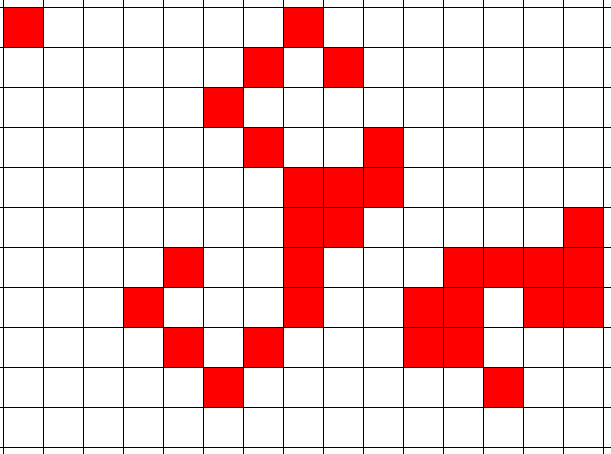
\includegraphics[scale=\myscale,scale=0.3]{ecran-vie-0}
\end{center} 

\insertvideo{7SR5-sUnotY}{Jeu de la vie}

\insertvideo{8d386Op5fsU}{Souris avec tkinter}

%%%%%%%%%%%%%%%%%%%%%%%%%%%%%%%%%%%%%%%%%%%%%%%%%%%%%%%%%%%%%%%%
%%%%%%%%%%%%%%%%%%%%%%%%%%%%%%%%%%%%%%%%%%%%%%%%%%%%%%%%%%%%%%%%

\begin{cours}[Règles du jeu de la vie]
Le \emph{jeu de la vie}\index{jeu de la vie} se déroule sur une grille. Chaque case peut contenir une cellule. Partant d'une configuration initiale, chaque jour des cellules vont naître et d'autres mourir en fonction du nombre de ses voisins.

Voici les règles :
\begin{itemize}
  \item Pour une case vide au jour $j$ et ayant exactement $3$ cellules voisines : une cellule naît au jour $j+1$.

\myfigure{0.5}{
  \tikzinput{fig-vie-0a}
}

  \item Pour une case contenant une cellule au jour $j$, ayant soit $2$ ou soit $3$ cellules voisines : alors la cellule continue de vivre.
  Dans les autres cas la cellule meurt (avec $0$ ou $1$, elle meurt d'isolement, avec plus de $4$ voisins, elle meurt de surpopulation !).
  
  \medskip
  
\myfigure{0.5}{
  \tikzinput{fig-vie-0b}
}  

   \medskip
    
\end{itemize}

Voici un exemple simple, le \og{}clignotant\fg{} :

\myfigure{0.5}{
  \tikzinput{fig-vie-0c}
} 
 
Voici un autre exemple (avec directement le nombre de voisins), la première évolution et l'évolution de l'évolution.

\myfigure{0.5}{
  \tikzinput{fig-vie-0d}
} 
\end{cours}



%%%%%%%%%%%%%%%%%%%%%%%%%%%%%%%%%%%%%%%%%%%%%%%%%%%%%%%%%%%%%%%%
% Activité 1
%%%%%%%%%%%%%%%%%%%%%%%%%%%%%%%%%%%%%%%%%%%%%%%%%%%%%%%%%%%%%%%%

\begin{activite}[Tableaux à deux dimensions]
\objectifs{Objectifs : définir et afficher des tableaux indexés par deux indices.}

Nous modélisons l'espace de vie des cellules par un tableau à double entrée, contenant des entiers, $1$ pour signifier la présence d'une cellule, $0$ sinon. Voici en exemple la configuration \og{}bouche\fg{} et son tableau :

\myfigure{0.6}{
  \tikzinput{fig-vie-1}
} 

\begin{enumerate}
  \item 
  \begin{itemize}
    \item Initialise deux variables \ci{n} (la hauteur du tableau) et \ci{p} (la largeur) (par exemple à $5$ et $8$).
    
    \item Définis un tableau à deux dimensions rempli de zéros par la commande :
    
    \centerline{\ci{tableau = [[0 for j in range(p)] for i in range(n)]}}
    
    \item Par des instructions du type \ci{tableau[i][j] = 1} remplis le tableau afin de définir la configuration du clignotant, de la bouche\ldots
  \end{itemize}
  
  \item Programme l'affichage à l'écran d'un tableau donné. 
  Par exemple, le clignotant s'affiche ainsi :
  
\begin{center}
\ci{00000000}\\
\ci{00000000}\\
\ci{00111000}\\
\ci{00000000}\\
\ci{00000000}
\end{center}

  \emph{Indication :} par défaut la commande \ci{print()} passe à la ligne suivante à chaque appel (il rajoute le caractère \ci{"\\n"} qui est le caractère de fin de ligne). On peut lui spécifier de ne pas le faire par l'option
  \ci{print("Mon texte",end="")}.
  
\end{enumerate}
\end{activite}



%%%%%%%%%%%%%%%%%%%%%%%%%%%%%%%%%%%%%%%%%%%%%%%%%%%%%%%%%%%%%%%%
% Activité 2
%%%%%%%%%%%%%%%%%%%%%%%%%%%%%%%%%%%%%%%%%%%%%%%%%%%%%%%%%%%%%%%%

\begin{activite}[Affichage graphique]

\objectifs{Objectifs : réaliser l'affichage graphique d'une configuration de cellules.}

\begin{center}
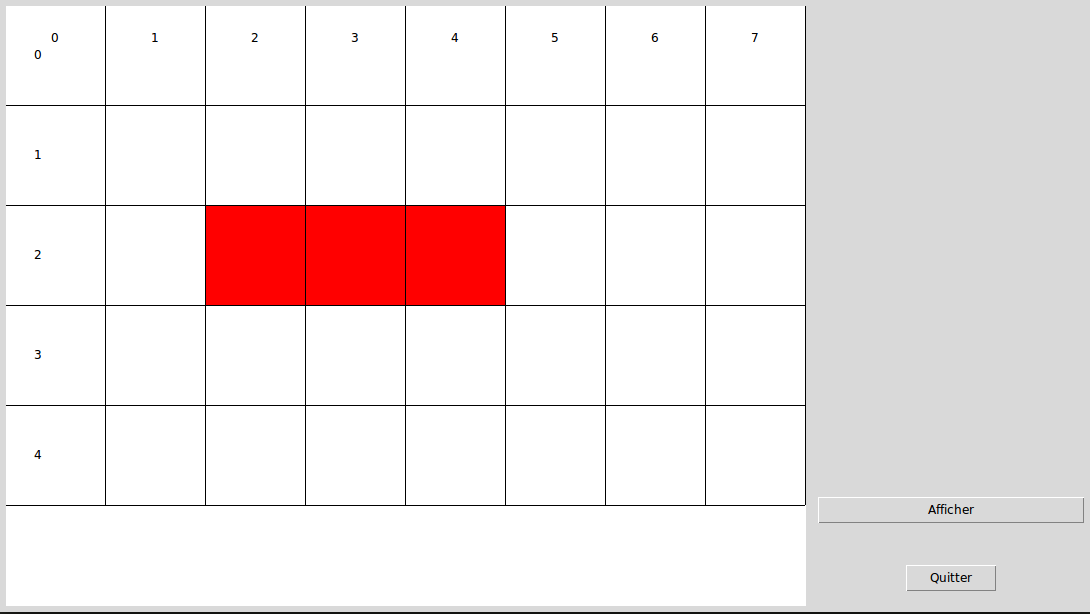
\includegraphics[scale=\myscale,scale=0.3]{ecran-vie-2}
\end{center} 

\begin{enumerate}
  \item Programme la création d'une fenêtre \ci{tkinter} (voir la fiche \og{}Statistique -- Visualisation de données\fg{}). Écris une fonction \ci{afficher_lignes()}, sans paramètre, qui affiche une grille vierge de coordonnées. Tu auras besoin d'une constante \ci{echelle} (par exemple \ci{echelle = 50}) pour transformer les indices $i$ et $j$ en des coordonnées graphiques $x$ et $y$, suivant la relation : $x= e \times j$ et $y = e \times i$ ($e$ étant l'échelle).
  
  \textbf{Bonus.} Tu peux aussi rajouter la valeur des indices $i$ et $j$ en haut et à gauche pour faciliter la lecture de la grille.
  
  \item Construis une fonction \ci{afficher_tableau(tab)} qui affiche graphiquement les cellules d'un tableau. 
  
  \textbf{Bonus.}  Rajoute un bouton \og{}Afficher\fg{} et un bouton \og{}Quitter\fg{}
(voir la fiche \og{}Statistique -- Visualisation de données\fg{}).  
  
\end{enumerate}
\end{activite}



%%%%%%%%%%%%%%%%%%%%%%%%%%%%%%%%%%%%%%%%%%%%%%%%%%%%%%%%%%%%%%%%
% Activité 3
%%%%%%%%%%%%%%%%%%%%%%%%%%%%%%%%%%%%%%%%%%%%%%%%%%%%%%%%%%%%%%%%

\begin{activite}[Évolution]

\objectifs{Objectifs : calculer l'évolution d'une configuration au jour d'après.}

\begin{enumerate}
  \item Programme une fonction \ci{nombre_voisins(i,j,tab)} qui calcule le nombre de cellules voisines vivantes de la cellule $(i,j)$.
  
  \emph{Indications.}
  \begin{itemize}
    \item Il y a en tout au maximum $8$ voisins possibles. Le plus simple est de les tester un par un !
    \item Pour le comptage, il faut faire bien attention aux cellules qui sont placées près d'un bord (et ont moins de $8$ voisins).
  \end{itemize}
  
  \item Programme une fonction \ci{evolution(tab)} qui en entrée reçoit un tableau et qui en sortie renvoie un nouveau tableau correspondant à la situation au jour d'après, selon les règles du jeu de la vie décrites au début.
 Par exemple, si le tableau de gauche correspond à l'entrée, alors la sortie correspond 
au tableau de droite :

\begin{center}
\begin{minipage}{0.3\textwidth}
\begin{center}
\ci{00000000}\\
\ci{00000000}\\
\ci{00111000}\\
\ci{00000000}\\
\ci{00000000}
\end{center}
\end{minipage} 
 évolue en  
\begin{minipage}{0.3\textwidth}
\begin{center}
\ci{00000000}\\
\ci{00010000}\\
\ci{00010000}\\
\ci{00010000}\\
\ci{00000000}
\end{center}
\end{minipage} 
\end{center}

  \emph{Indications.} Pour définir un nouveau tableau reprend la commande :
  
      \centerline{\ci{nouveau_tableau = [[0 for j in range(p)] for i in range(n)]}}
      
  puis modifie le tableau comme voulu.

\end{enumerate}
\end{activite}


 

%%%%%%%%%%%%%%%%%%%%%%%%%%%%%%%%%%%%%%%%%%%%%%%%%%%%%%%%%%%%%%%%
% Activité 4
%%%%%%%%%%%%%%%%%%%%%%%%%%%%%%%%%%%%%%%%%%%%%%%%%%%%%%%%%%%%%%%%

\begin{activite}[Itérations]

\objectifs{Objectifs : finir le programme graphique afin que l'utilisateur puisse définir des configurations et les faire évoluer d'un simple clic.}

\begin{enumerate}
  \item  Améliore la fenêtre graphique afin de faciliter la vie de l'utilisateur :
  \begin{itemize}
    \item Un bouton \og{}évoluer\fg{} qui à chaque clic affiche l'évolution.
    \item Des boutons permettant d'afficher des configurations pré-définies (sur la capture d'écran ci-dessous c'est la configuration \og{}pentadecathlon\fg{}).
  \end{itemize}
  
\begin{center}
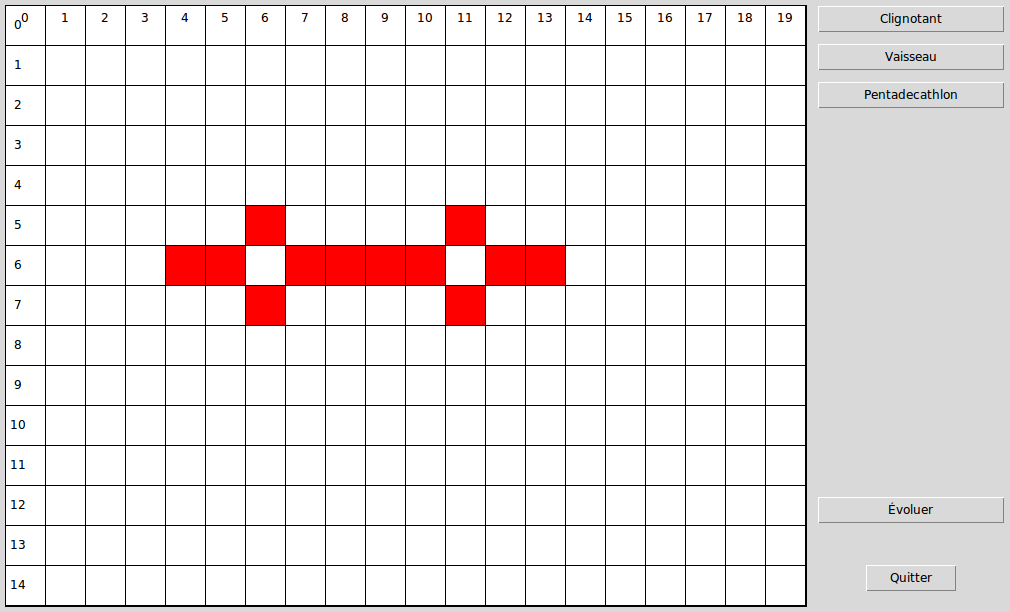
\includegraphics[scale=\myscale,scale=0.3]{ecran-vie-4a}
\end{center}  
  
  \item Perfectionne ton programme afin que l'utilisateur dessine la configuration qu'il souhaite par des clics de la souris. Un clic sur une case éteinte l'allume, un clic sur une case allumée l'éteint. 
  Tu peux décomposer ce travail en trois fonctions :
  \begin{itemize}
    \item \ci{allumer_eteindre(i,j)}, qui commute la cellule $(i,j)$ ;
    \item \ci{xy_vers_ij(x,y)} qui convertit des coordonnées graphiques $(x,y)$ en des coordonnées entières $(i,j)$ (utiliser la variable \ci{echelle} et la division entière).
    \item \ci{action_clic_souris(event)} pour récupérer les coordonnées $(x,y)$ d'un clic de souris (voir le cours ci-dessous) et commuter la case cliquée.
  \end{itemize}   
    
\begin{center}
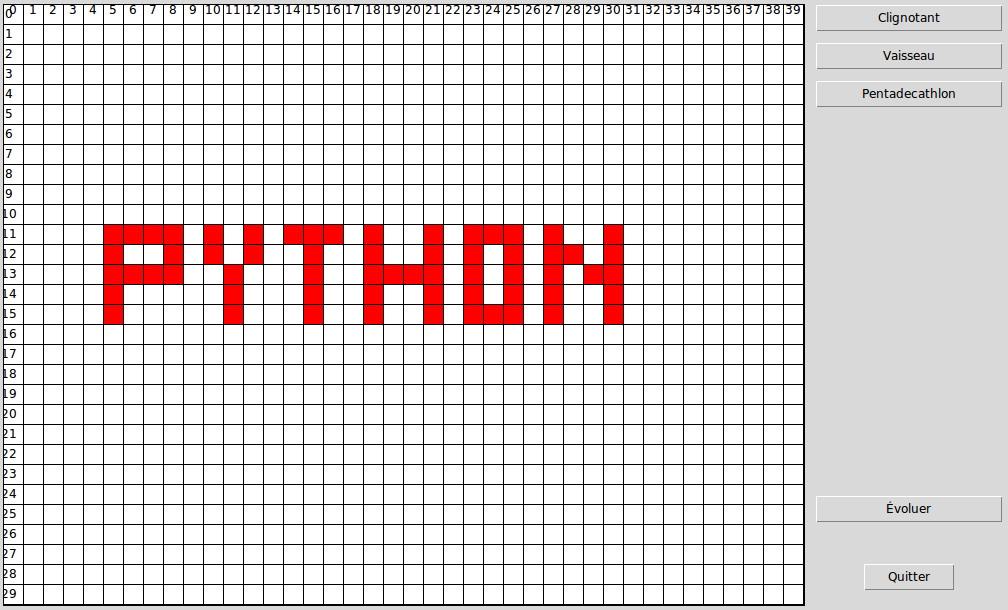
\includegraphics[scale=\myscale,scale=0.3]{ecran-vie-4b}
\end{center}

    
\end{enumerate}
\end{activite} 


\begin{cours}[Clic de souris]

\index{tkinter@\ci{tkinter}}
\index{module!tkinter@\ci{tkinter}}
\index{souris}
\index{clic}

Voici un petit programme qui affiche une fenêtre graphique. Chaque fois que l'utilisateur clique (avec le bouton gauche de la souris) le programme affiche un petit carré (sur la fenêtre) et affiche \og{}Clic à $x=\ldots$, $y=\ldots$\fg{} (sur la console).

\begin{lstlisting}
from tkinter import *

# Fenêtre
root = Tk()
canvas = Canvas(root, width=800, height=600, background="white")
canvas.pack(side=LEFT, padx=5, pady=5)

# Capture des clics de souris
def action_clic_souris(event):
    canvas.focus_set()
    x = event.x
    y = event.y
    canvas.create_rectangle(x,y,x+10,y+10,fill="red")
    print("Clic à x =",x,", y =",y)
    return

# Association clic/action
canvas.bind("<Button-1>", action_clic_souris)

# Lancement
root.mainloop()
\end{lstlisting}


Voici quelques explications :
\begin{itemize}
  \item La création de la fenêtre est habituelle. Le programme se termine par le lancement avec la commande \ci{mainloop()}.
  
  \item Le premier point clé est d'associer un clic de souris à une action, c'est ce que fait la ligne 
  
\centerline{\ci{canvas.bind("<Button-1>", action_clic_souris)}}

Chaque fois que le bouton gauche de la souris est cliqué, \Python{} exécute la fonction \ci{action_clic_souris}. (Note qu'il n'y a pas de parenthèses pour l'appel à la fonction.)

   \item Second point clé : la fonction \ci{action_clic_souris} récupère les coordonnées du clic et ici ensuite fait deux choses : elle affiche un petit rectangle à l'endroit du clic et affiche dans la fenêtre du terminal les coordonnées $(x,y)$.
   
   \item Les coordonnées $x$ et $y$ sont exprimées en pixels ; $(0,0)$ désigne le coin en haut à gauche de la fenêtre (la zone délimitée par \ci{canvas}).
\end{itemize}
\end{cours}



Voici quelques idées pour aller plus loin :
\begin{itemize}
  \item Fais en sorte que la grille s'adapte automatiquement à la largeur de l'écran, c'est-à-dire calcule \ci{echelle} en fonction de \ci{n} et \ci{p}.
  
  \item Rajoute une étape intermédiaire avant d'évoluer : colorie en vert une cellule qui va naître et en noir une cellule qui va mourir. Pour cela les éléments de \ci{tableau} pourront prendre des valeurs autres que $0$ et $1$.
\end{itemize}

Voici quelques configurations intéressantes. 
\myfigure{0.6}{
  \tikzinput{fig-vie-4a} \quad 
  \tikzinput{fig-vie-4b} 
} 

Tu en trouveras plein d'autres sur internet mais surtout amuse-toi à en découvrir de nouvelles !

En particulier, trouve des configurations :
\begin{itemize}
  \item qui restent fixes au cours du temps ;
  \item qui évoluent, puis deviennent fixes ;
  \item qui sont périodiques (les mêmes configurations reviennent en boucles) avec une période de $2$, $3$ ou plus ;
  \item qui voyagent ;
  \item qui propulsent des cellules ; 
  \item dont la population augmente indéfiniment !
\end{itemize}


\end{document}
